
\chapter{Brownian Motion}


\section{Historical observations}
The history of Brownian motion dates back to the early observations of the botanist Robert Brown. While observing pollen grains suspended in a liquid, he noted their highly erratic and jagged trajectory. These particles were subsequently named \textit{Brownian} particles.


\begin{figure}[h!]
    \centering
    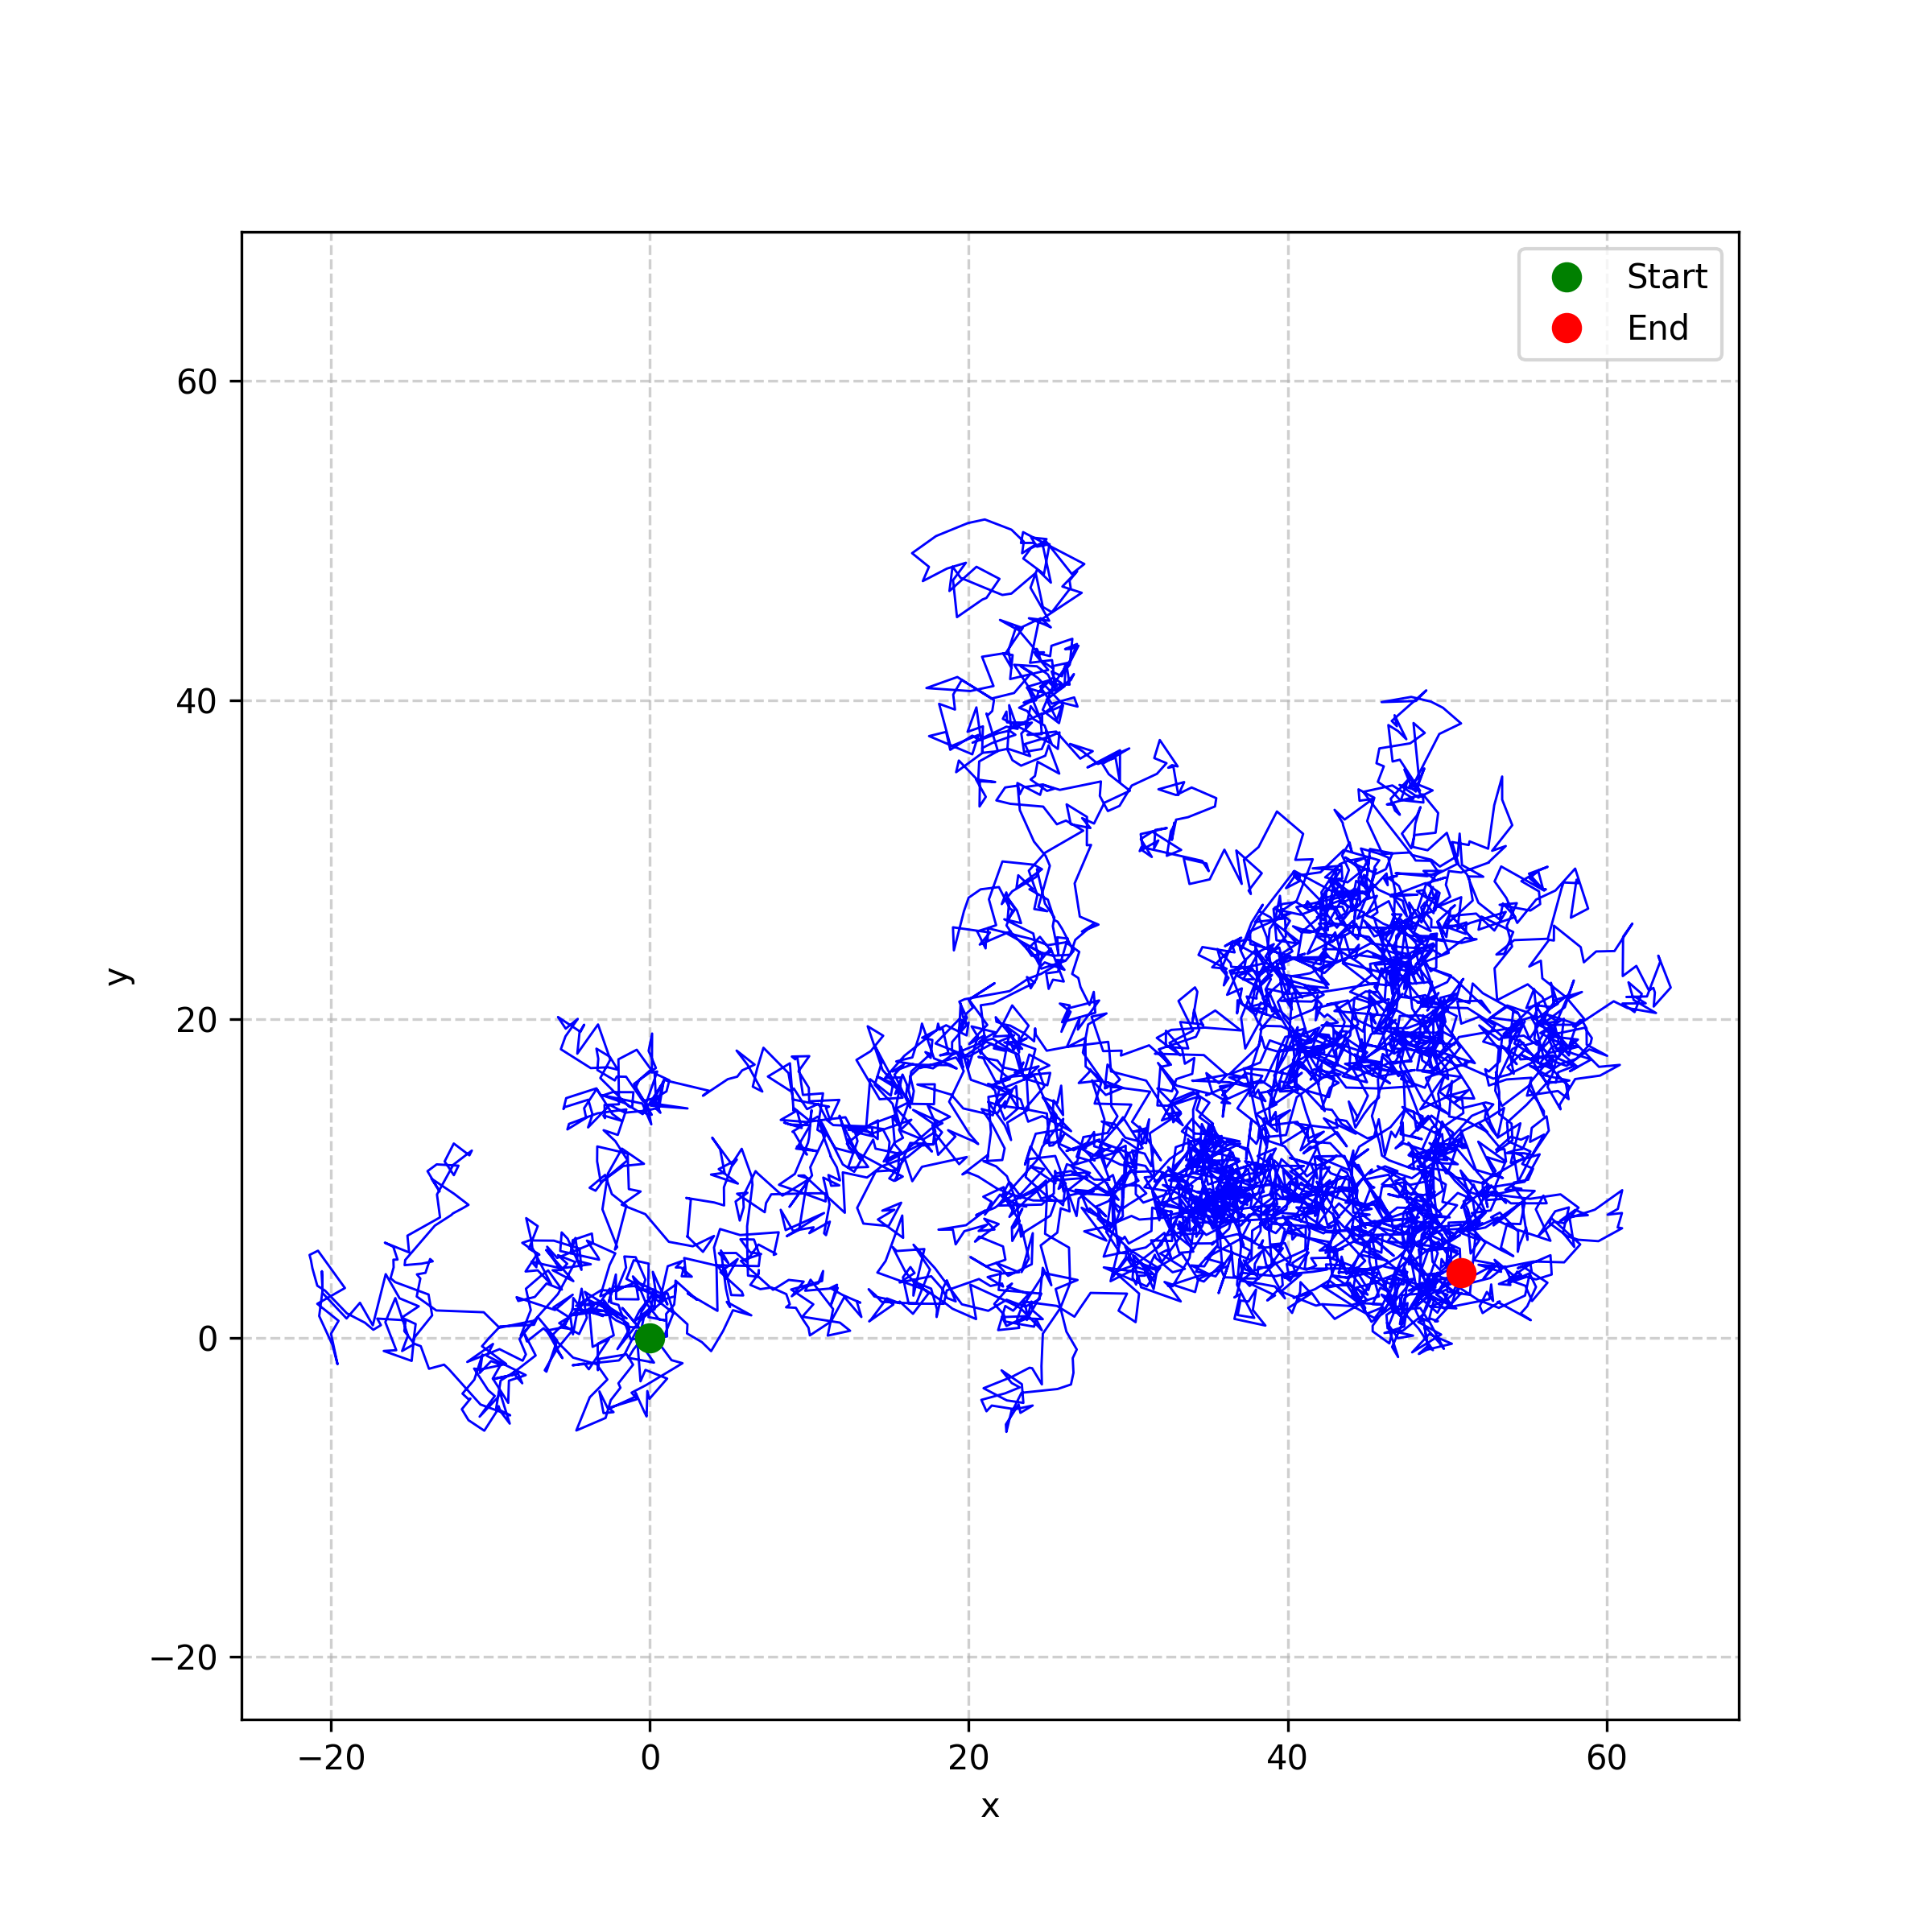
\includegraphics[width=0.6\textwidth]{images/brownian_motion_2d.png} 
    \caption{Simulation of a Brownian trajectory in two dimensions.}
\end{figure}

Specifically, Brown made the following qualitative observations:
\begin{enumerate}[label=\roman*)]
    \item The motion never seems to cease.
    \item Different particles always move independently of one another.
    \item The particle's material composition (organic or inorganic) or its mass density do not seem to matter.
    \item The motion becomes faster and more agitated as the fluid's temperature increases or as its viscosity decreases.
    \item The motion exhibits scale invariance (it looks similarly jagged at different magnifications).
    \item The trajectory appears to have no tangent at any point.
\end{enumerate}

The first theoretical characterization of this phenomenon was provided by Albert Einstein in two revolutionary papers published in 1905 \cite{Einstein1905, Einstein1906}. We will now illustrate the key steps of his reasoning.
\section{Einstein's first paper}
\subsection{From random walk to the diffusion equation}
He considered a one-dimensional, infinitely extended fluid composed of an ensemble of particles. The Brownian particle undergoes a series of discrete displacements, or "jumps", over very small, successive time intervals, denoted by $\tau$, much smaller than the observation time $T$.


\begin{center}
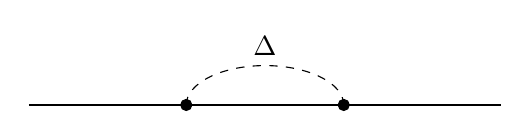
\begin{tikzpicture}

  \draw[thick] (-3,0) -- (3,0);

  \filldraw[black] (-1,0) circle (2pt);
  \filldraw[black] (1,0) circle (2pt);

  \draw[dashed] (-1,0) arc (180:0:1cm and 0.5cm);

  \node[above] at (0,0.5) {$\Delta$};
\end{tikzpicture}
\end{center}

To describe the statistics of these jumps, Einstein introduced an auxiliary function, $\phi(\Delta)$, which is the probability density function (PDF) for a jump of magnitude $\Delta$. The term $\phi(\Delta)d\Delta$ represents the probability that a single jump has a magnitude between $\Delta$ and $\Delta+d\Delta$. This function is defined by two fundamental properties based on physical reasoning:
\begin{itemize}
    \item \textbf{Normalization}: The particle must perform a jump of some magnitude, so the total probability over all possible jumps must be equal to 1. This is expressed by the normalization condition:
    \[
    \int_{-\infty}^{\infty} \phi(\Delta) \,d\Delta = 1.
    \]
    \item \textbf{Symmetry}: In the absence of any external force or drift, the fluid is isotropic. Therefore, a jump to the right ($+\Delta$) is as probable as a jump of the same magnitude to the left ($-\Delta$). This implies that the function $\phi$ must be an even function:
    \[
    \phi(\Delta) = \phi(-\Delta).
    \]
\end{itemize}

The main goal, however, is to find $p(x,t)$, which represents the number of particles per unit length at position $x$ and time $t$. If we consider $p(x,t)$ as the probability density for a single particle, it must be normalized such that its integral over all space is 1:
\[
\int_{-\infty}^{\infty} p(x,t) \,dx = 1.
\]
The probability of finding the particle in the infinitesimal interval $[x, x+dx]$ is therefore $p(x,t)dx$.

The core idea is to relate the particle density at time $t_f = t+\tau$ to the density at time $t_i = t$. The density of particles at position $x$ at the future time $t+\tau$, denoted $p(x, t+\tau)$, is the sum of probabilities of particles arriving at $x$ from all possible previous positions. A particle that ends up at $x$ must have been at a position $x+\Delta$ at time $t$ and then performed a jump of size $\Delta$. Summing over all possible jumps $\Delta$:
\[
p(x, t+\tau) = \int_{-\infty}^{\infty} P(x+\Delta, t) \phi(\Delta) \,d\Delta.
\]

Now, we perform a Taylor expansion for small $\tau$ and small $\Delta$. The left side is expanded in time:
\[
p(x, t+\tau) \approx p(x,t) + \tau \frac{\partial p(x,t)}{\partial t} + \dots;
\]
the term $p(x+\Delta, t)$ inside the integral is expanded in space around the position $x$:
\[
p(x+\Delta, t) \approx p(x,t) + \Delta \frac{\partial p(x,t)}{\partial x} + \frac{\Delta^2}{2} \frac{\partial^2 p(x,t)}{\partial x^2} + \dots;
\]
s3ubstituting these expansions back into the main equation:
\[
p(x,t) + \tau \frac{\partial P}{\partial t} \approx \int_{-\infty}^{\infty} \left[ p(x,t) + \Delta \frac{\partial p}{\partial x} + \frac{\Delta^2}{2} \frac{\partial^2 p}{\partial x^2} \right] \phi(\Delta) \,d\Delta.
\]
We can split the integral by linearity:
\[
\tau \frac{\partial p}{\partial t} \approx p(x,t) \underbrace{\int \phi(\Delta)d\Delta}_{=1} + p(x,t) + \frac{\partial p}{\partial x} \underbrace{\int \Delta \phi(\Delta)d\Delta}_{=0} + \frac{1}{2}\frac{\partial^2 p}{\partial x^2} \int \Delta^2 \phi(\Delta)d\Delta.
\]
The terms simplify based on the properties of $\phi$.

So we are left with:
\[
\tau \frac{\partial p(x,t)}{\partial t} \approx \frac{1}{2}\frac{\partial^2 p(x,t)}{\partial x^2} \int_{-\infty}^{\infty} \Delta^2 \phi(\Delta) \,d\Delta.
\]
Dividing by $\tau$, we get:
\[
\frac{\partial p(x,t)}{\partial t} = D \frac{\partial^2 p(x,t)}{\partial x^2}.
\]
This is the \emph{diffusion equation} (with $D=1$ it becomes the well known heat equation), where $D$ is the \emph{diffusion coefficient}, defined as:
\[
D := \frac{1}{2\tau} \int_{-\infty}^{\infty} \Delta^2 \phi(\Delta) \,d\Delta.
\]
Since $\Delta^2 \ge 0$ and $\phi(\Delta) \ge 0$, the integral is positive, thus $D>0$. The dimensions of $D$ are length squared per unit time, $[D] = L^2 T^{-1}$.


\subsection{Solution of the diffusion equation}
We now solve the diffusion equation with a specific initial condition. Physically, it is natural to assume that the process starts with the particle (or all particles) located exactly at the origin at time $t=0$. This condition is represented mathematically by the Dirac delta function, $\delta(x)$. It represents an instantaneous, infinitely concentrated point source. The solution $p(x,t)$ will then describe how this initial certainty "diffuses" into a probability distribution over time.

The problem is thus defined by the partial differential equation and its initial condition:
\begin{align*}
    \frac{\partial p(x,t)}{\partial t} &= D \frac{\partial^2 p(x,t)}{\partial x^2}; \\
    p(x,0) &= \delta(x).
\end{align*}
We solve this using the Fourier transform. Let $p(k,t)$ be the Fourier transform of $p(x,t)$ with respect to the spatial variable $x$. The transform pair is defined as:
\begin{align*}
    \text{Inverse Transform:} \quad p(x,t) &= \int_{-\infty}^{\infty} e^{ikx} p(k,t) \,dk; \\
    \text{Transform:} \quad p(k,t) &= \frac{1}{2\pi} \int_{-\infty}^{\infty} e^{-ikx} p(x,t) \,dx.
\end{align*}
First, we transform the initial condition. Using the integral representation of the Dirac delta, $\delta(x) = \frac{1}{2\pi} \int e^{ikx} dk$,  
\[
p(k,0) = \frac{1}{2\pi}.
\]
Next, we transform the diffusion equation itself. The time derivative remains, while the spatial derivative becomes a multiplication by $(ik)^2 = -k^2$:
\[
\mathcal{F}\left[\frac{\partial p}{\partial t}\right] = D \cdot \mathcal{F}\left[\frac{\partial^2 p}{\partial x^2}\right] \implies \frac{\partial p(k,t)}{\partial t} = D(-k^2)p(k,t).
\]
This transforms the partial differential equation in $(x,t)$ into a simpler ordinary differential equation in the variable $t$ for each value of $k$:
\begin{align*}
    \frac{\partial p(k,t)}{\partial t} &= -Dk^2 p(k,t); \\
    p(k,0) &= \frac{1}{2\pi}.
\end{align*}
This is a first-order linear ODE with constant coefficients, which can be solved by separation of variables.

Let's treat $k$ as a constant parameter and solve the ODE for the function $f(t) = p(k,t)$:
\[
\frac{df(t)}{dt} = (-Dk^2) f(t).
\]
Separating the variables $f$ and $t$:
\[
\frac{df}{f} = -Dk^2 \,dt.
\]
Integrating both sides:
\[
\int \frac{1}{f} \,df = \int -Dk^2 \,dt \implies \ln|f| = -Dk^2 t + C_0.
\]
where $C_0$ is the constant of integration. Exponentiating both sides gives:
\[
f(t) = e^{-Dk^2 t + C_0} = e^{C_0} e^{-Dk^2 t} = C e^{-Dk^2 t}.
\]
We find the constant $C$ using the initial condition $p(k,0) = 1/(2\pi)$:
\[
p(k,0) = C e^{0} = C \implies C = \frac{1}{2\pi}.
\]
Thus, the solution in the Fourier space is:
\[
p(k,t) = \frac{1}{2\pi} e^{-Dk^2 t}.
\]

To find the solution in the original space, we apply the inverse Fourier transform to $p(k,t)$:
\[
p(x,t) = \int_{-\infty}^{\infty} e^{ikx} p(k,t) \,dk = \frac{1}{2\pi} \int_{-\infty}^{\infty} e^{ikx} e^{-Dk^2 t} \,dk = \frac{1}{2\pi} \int_{-\infty}^{\infty} e^{-Dk^2 t + ikx} \,dk.
\]
To solve this Gaussian integral, we complete the square in the exponent:
\begin{align*}
-Dtk^2 + ikx &= -Dt \left( k^2 - \frac{ix}{Dt}k \right) \\
             &= -Dt \left[ \left( k - \frac{ix}{2Dt} \right)^2 - \left( \frac{ix}{2Dt} \right)^2 \right] \\
             &= -Dt \left( k - \frac{ix}{2Dt} \right)^2 - Dt \left( \frac{x^2}{4D^2t^2} \right) \\
             &= -Dt \left( k - \frac{ix}{2Dt} \right)^2 - \frac{x^2}{4Dt}.
\end{align*}
Substituting this back into the integral:
\[
p(x,t) = \frac{1}{2\pi} \int_{-\infty}^{\infty} \exp\left[-Dt\left(k - \frac{ix}{2Dt}\right)^2 - \frac{x^2}{4Dt}\right] \,dk = \frac{1}{2\pi} e^{-\frac{x^2}{4Dt}} \int_{-\infty}^{\infty} e^{-Dt\left(k - \frac{ix}{2Dt}\right)^2} \,dk.
\]
The remaining integral is a standard Gaussian integral of the form $\int e^{-a(u-b)^2}du = \sqrt{\pi/a}$. Here, $a=Dt$. The complex shift $b=ix/(2Dt)$ does not change the result of the integral over the real line.
\[
\int_{-\infty}^{\infty} e^{-Dt\left(k - \frac{ix}{2Dt}\right)^2} \,dk = \sqrt{\frac{\pi}{Dt}}.
\]
Therefore, the solution is:
\[
p(x,t) = \frac{1}{2\pi} e^{-\frac{x^2}{4Dt}} \sqrt{\frac{\pi}{Dt}} = \frac{1}{\sqrt{4\pi Dt}} e^{-\frac{x^2}{4Dt}}.
\]
This is a Gaussian distribution with mean $\mu=0$ and variance $\sigma^2_t = 2Dt$.

A minimal and standard choice for the diffusion coefficient is $D=1/2$. This specific case defines the standard Brownian motion, also known as the \emph{Wiener process}. The probability density function becomes:
\[
p(x,t) = \frac{1}{\sqrt{2\pi t}} e^{-\frac{x^2}{2t}}.
\]
This process is a cornerstone of stochastic calculus. It exhibits scale invariance and is considered the first and most fundamental example of a 1D fractal process.


\subsection{Physical interpretation and statistical consequences}
The solution we found is a  normal distribution:
\[
p(x,t) = \frac{1}{\sqrt{2\pi\sigma_t^2}} e^{-\frac{x^2}{2\sigma_t^2}}.
\]
where the variance $\sigma_t^2$ is time-dependent:
\[
\sigma_t^2 = 2Dt.
\]


We can calculate the key moments of this distribution.
\begin{itemize}
    \item \textbf{Mean Position}: The average position of the particle is given by the expectation value $\langle x \rangle$. Since the Gaussian is centered at zero (it is an even function) and we are integrating over a symmetric domain, the mean is zero.
    \[
    \langle x \rangle = \int_{-\infty}^{\infty} x \, p(x,t) \,dx = 0.
    \]
    This confirms that the diffusion process has no drift; the particle is equally likely to be found on either side of the origin.

    \item \textbf{Variance}: The variance measures the spread of the distribution.
    \begin{align*}
        \text{Var}[x] &= \langle (x - \langle x \rangle)^2 \rangle = \langle x^2 \rangle - \langle x \rangle^2 = \langle x^2 \rangle \\
        &= \int_{-\infty}^{\infty} x^2 \, p(x,t) \,dx = \sigma_t^2 = 2Dt.
    \end{align*}
    This is a very important result of diffusion theory: the variance of the particle's position grows linearly with time. This means the particle spreads out, and our uncertainty about its location increases as time passes. Standard diffusive processes are thus Gaussian.
\end{itemize}

The evolution of the probability density is a macroscopic description of the ensemble of particles, not the path of a single particle. It starts as an infinitely sharp Dirac delta at $t=0$ and then "spreads out" as a Gaussian with increasing width, as illustrated below.

\begin{figure}[h!]
    \centering
    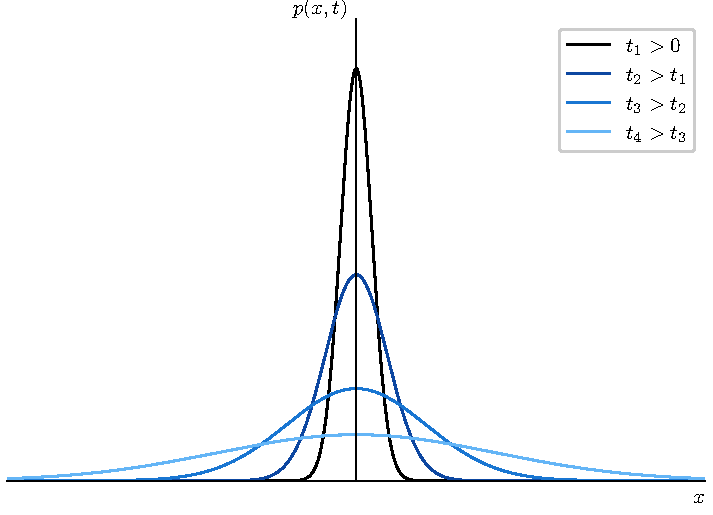
\includegraphics[width=0.8\textwidth]{images/gaussian_evolution.pdf}
    \caption{Evolution of the probability density $p(x,t)$ over time. Starting from a Dirac delta at $t=0$, the distribution spreads out as a Gaussian with variance $\sigma_t^2=2Dt$ increasing linearly in time.}
    \label{fig:gaussian_evolution}
\end{figure}


Another relevant quantity to characterize the displacement of the particle is the Mean Squared Displacement (MSD). It is defined as the average squared distance the particle has traveled from its starting point.
\[
\text{MSD}(t) = \langle [x(t) - x(0)]^2 \rangle.
\]
Let's consider two cases:
\begin{itemize}
    \item If the particle starts at the origin, $x(0)=0$:
    \[
    \text{MSD} = \langle [x(t)]^2 \rangle = \langle x^2(t) \rangle = 2Dt.
    \]
    The MSD is simply the variance.

    \item If the particle starts at a generic position $x(0)=x_0$: 
    \begin{align*}
        \text{MSD} &= \langle [x(t) - x_0]^2 \rangle \\
        &= \langle x^2(t)\rangle + x_0^2 - 2x_0  \langle x(t)\rangle\\
        &= \langle x^2(t)\rangle + x_0^2 - 2x_0^2  \\
        & = x_0^2  + 2Dt - x_0^2 \\
        & = 2Dt.
    \end{align*}
\end{itemize}
In both cases, the MSD grows linearly with time. 

The typical distance traveled by the particle, the mean free path  $\lambda_x$, can be estimated as the root of the MSD.
\[
\lambda_x = \sqrt{\text{MSD}} = \sqrt{2Dt}.
\]
This shows that the characteristic displacement of a diffusing particle grows not with time $t$, but with its square root. This sub-linear growth is a direct consequence of the random, back-and-forth nature of the motion.

\section{Einstein's second paper}

